%%%%%%%% ICML 2018 EXAMPLE LATEX SUBMISSION FILE %%%%%%%%%%%%%%%%%

\documentclass{article}

% Recommended, but optional, packages for figures and better typesetting:
\usepackage{microtype}
\usepackage{graphicx}
\usepackage{subfigure}
\usepackage{booktabs} % for professional tables
\usepackage{amsmath, amssymb}

\usepackage[utf8]{inputenc}
\usepackage[T1]{fontenc}
\usepackage{hyperref}
\usepackage{url}
\usepackage{booktabs}
\usepackage{amsfonts}
\usepackage{nicefrac}
\usepackage{microtype}
\usepackage{xcolor}
\usepackage{lipsum}
% \usepackage[nomarkers,nolists,figuresonly]{endfloat} %comment out when finish
\usepackage{booktabs}
\usepackage{multirow}
\usepackage{float}
\usepackage{subcaption}


% hyperref makes hyperlinks in the resulting PDF.
% If your build breaks (sometimes temporarily if a hyperlink spans a page)
% please comment out the following usepackage line and replace
% \usepackage{icml2018} with \usepackage[nohyperref]{icml2018} above.
\usepackage{hyperref}

% Attempt to make hyperref and algorithmic work together better:
\newcommand{\theHalgorithm}{\arabic{algorithm}}

% Use the following line for the initial blind version submitted for review:
\usepackage[accepted]{icml2018}

% If accepted, instead use the following line for the camera-ready submission:
%\usepackage[accepted]{icml2018}

% The \icmltitle you define below is probably too long as a header.
% Therefore, a short form for the running title is supplied here:
\icmltitlerunning{CS234: Reinforcement Learning Winter 2025 - Final Project Milestone}

\begin{document}

%%%%%%%%%%%%%%%%%%%%%%%%%%%%%%%%%%%%%%%%%%%%%%%%%%%%%%%%%%%%%%%%
%%%%%%%%%%%          HEADER SECTIONS HERE            %%%%%%%%%%%
%%%%%%%%%%%%%%%%%%%%%%%%%%%%%%%%%%%%%%%%%%%%%%%%%%%%%%%%%%%%%%%%


\twocolumn[
\icmltitle{Enhancing Game Control Through \\
Hybrid Reinforcement Learning
}

\begin{icmlauthorlist}
\icmlauthor{Danhua Yan}{to}
\end{icmlauthorlist}

\icmlaffiliation{to}{Department of Computer Science, Stanford University}
\icmlcorrespondingauthor{Danhua Yan}{dhyan@stanford.edu}

% You may provide any keywords that you
% find helpful for describing your paper; these are used to populate
% the "keywords" metadata in the PDF but will not be shown in the document
% \icmlkeywords{Machine Learning, ICML}

\vskip 0.3in
]

% this must go after the closing bracket ] following \twocolumn[ ...

% This command actually creates the footnote in the first column
% listing the affiliations and the copyright notice.
% The command takes one argument, which is text to display at the start of the footnote.
% The \icmlEqualContribution command is standard text for equal contribution.
% Remove it (just {}) if you do not need this facility.

%\printAffiliationsAndNotice{}  % leave blank if no need to mention equal contribution
% \printAffiliationsAndNotice{\icmlEqualContribution} % otherwise use the standard text.
\printAffiliationsAndNotice{} % otherwise use the standard text.



%%%%%%%%%%%%%%%%%%%%%%%%%%%%%%%%%%%%%%%%%%%%%%%%%%%%%%%%%%%%%%%%
%%%%%%%%%%%           MAIN SECTIONS HERE             %%%%%%%%%%%
%%%%%%%%%%%%%%%%%%%%%%%%%%%%%%%%%%%%%%%%%%%%%%%%%%%%%%%%%%%%%%%%


% \begin{abstract}
% This document provides a basic paper template and submission guidelines.
% Abstracts must be a single paragraph, ideally between 4--6 sentences long.
% Gross violations will trigger corrections at the camera-ready phase.
% \end{abstract}

\section{Introduction}

% What is the problem that you will be investigating ? Why is it interesting ?
% What literature have you already surveyed or will be 
% examining to provide context and background ?

Training Reinforcement Learning (RL) agents usually requires a substantial 
amount of data and exploration to find an optimal policy. In many complex 
games, the challenges of high-dimensional state spaces, sparse rewards, and 
complex dynamics make training agents using pure exploration particularly 
inefficient. Moreover, in cases where exploration opportunities are limited or 
costly, the RL agent might fail to learn any usable policies \cite{Coletti2023EffectivenessOW}. 
Such inefficiency not only slows down learning but also increases the risk of 
converging to policies that are far from optimal.

The research field of bootstrapping an RL agent's policy from demonstrations or 
imitation learning shows significant promise. Various hybrid paradigms that 
combine human guidance as offline RL and agent exploration as online RL have 
shown they can accelerate policy learning and achieve above-demonstration 
performance \cite{hester_dqfd_2017,nair_bcrl_overcoming_2018, song_hybrid_2023, 
ren_hybrid_2024, Coletti2023EffectivenessOW}.

This project investigates how hybrid RL (HRL) can effectively enhance game control 
through guided explorations of the agent. It aims to evaluate the potential for 
achieving performance that surpasses the demonstration level.

\section{Approach}
\subsection{Environement}
In this project, we leverage the \texttt{stable-retro} library to create an OpenAI Gym 
environment for training an agent to play the NES game Super Mario Bros, level 1-1. The 
default integration of the environment encapsulates the game into the in-game visual 
frame as a matrix $I \in \mathbb{R}^{H \times W \times 3}$, where each element takes an 
integer value between 0 and 255, representing the RGB channels of the frame. The action 
of pressing 9 buttons on NES controllers is represented as a vector 
$\mathbf{a} = (a_1, a_2, \dots, a_9) \in \{0, 1\}^9$, where each button can be toggled 
independently, resulting in a total of 512 discrete action spaces. The default reward 
is the change in the $x$-axis position $\Delta x$ moved by Mario. In-game metadata, including 
scores, time left, and positions of Mario, can also be retrieved for each timestep $t$.

To record human demonstrations, we implemented scripts that save the gameplay 
through interactions with the environment, controlled via a game controller. 
The trajectory data of each episode $i$ is saved as $\tau_{hd}^{i} = \{(s_t, a_t, 
r_t, d_t, m_t)\}_{t=0}^{T}$, where each element in the tuple represents the 
state, action, reward, termination boolean, and metadata. We recorded five 
gameplays by amateur players, each successfully finishing Level 1-1 without 
losing a life of Mario.

To frame the game into a proper RL problem that can be solved within a
reasonable time, we made below custom modifications to the default integration
of the game:

\textbf{Action Space} 
The default 512 discrete action space captures all possible joystick button 
combinations. However, most of these combinations are not meaningful for 
controlling Mario. From the human demonstration trajectories, we narrowed down 
the action space to 10 common used button combinations (see 
Appendix \ref{a1:custom_env}).

\textbf{Termination States}
The default termination of the game occurs either when Mario has exhausted all 
his lives (3 to start with) or when the time limit of 400 seconds for Level 1-1 is reached. This 
setting poses challenges for RL exploration, as it may take too long to wait 
for the game to finish if Mario gets stuck at some point. We employ a stricter 
termination state: 1) Mario has only one life, and the game terminates 
immediately if he loses it; 2) If Mario remains stuck at the same position 
without moving to the right for 10 seconds, the game is terminated.

\textbf{Reward Function}
The default reward function is simply $\mathcal{R} = \min(0,\Delta x)$, which 
awards Mario for moving right and does not penalize for moving left. To 
incorporate other elements of the game, such as collecting coins, power-ups, 
defeating enemies, and to penalize Mario for not moving or losing the game, we 
adjust the reward function as follows: 
$\mathcal{R} = \min(0,\Delta x) + \Delta k - \Delta \text{t} - \mathbf{1}[d_t = 1] p$, 
where $\Delta k$ is the score earned since the last state, $\Delta \text{t}$ is 
the time spent in seconds since the last state, and $p$ is the penalty for 
terminating the game without successfully reaching the destination.


\subsection{Policy Network Archetectures}

For comparisons, all baselines and HRL approaches will leverage the same 
architecture of a convolutional neural network $\pi(s,a;\theta)$ that maps an RGB image of 
dimensions \(H \times W \times 3\) to a discrete action space of 10 actions. 
The architecture consists of three convolutional layers, with 16, 32, and 64 
hidden channels respectively. Each convolution uses a \(3 \times 3\) kernel 
with stride $1$ and padding $1$, followed by a ReLU activation and \(2 \times 
2\) max pooling that halves the spatial dimensions. The output feature maps 
are flattened into a vector, then processed by a fully connected hidden layer 
with 512 units and ReLU activation. Finally, a linear output layer projects 
the 512-dimensional representation to 10 logits corresponding to the available 
actions.
All models are trained using the AdamW optimizer with default settings from 
PyTorch, and a learning rate of $10^{-4}$ unless otherwise specified.

\subsection{Baselines}
Here we shall establish performance of offline-only and online-only RL approaches
as baselines to compare against future HRL approaches and human demonstration trajectories. 

\subsubsection{Deep \textit{Q}-Learning (DQN)}

Here we use the DQN architecture with a linearly decaying $\epsilon$-greedy 
exploration as a baseline for the online RL approach through pure explorations. 
We implemented the DQN architecture from scratch to facilitate future 
modifications for the HRL approach DQfD.

We set the DQN parameters as follows: the discount factor $\gamma=0.99$. The 
replay buffer has a capacity of $|\mathcal{D}|=10000$, where new states 
overwrite old states in a FIFO manner. The policy is trained for 2500 episodes, 
with the target policy network updated after each episode.

We made a minor modification to the classic DQN algorithm: instead of sampling 
a minibatch of samples and updating the policy network $\pi(s,a;\theta)$ for 
every $t$, we set a parameter $\omega$ that allows the agent to interact with 
the environment for $\omega$ steps before updating $\pi(s,a;\theta)$. The 
rationale is that in Super Mario Bros, after an action is played, especially 
for a jump, there is a brief period during which no actions can be controlled. 
Thus, adding such frames to the replay buffer becomes inefficient for updates 
without meaningful new information. $\omega$ is empirically set to 50, which is 
approximately under 1 second in a 60 fps game setting. $\epsilon$ is decayed 
from 1 to 0.01 linearly, scaled by episodes interacted during the training 
process.

\subsubsection{Behavior Cloning (BC)}
Behavioral cloning (BC) is an offline-only approach that uses supervised 
learning to map state-action pairs from human demonstration trajectories. We 
recorded five successful trajectories from amateur players, and each episode 
$i$ is saved as $\tau_{hd}^{i} \{(s_t, a_t, r_t, d_t, m_t)\}_{t=0}^{T}$. All 
$(s_t, a_t)$ pairs are randomly split into \texttt{train} and \texttt{dev} sets 
in a 7:3 ratio. With a batch size of 32 and cross-entropy loss function, the 
policy network $\pi(s,a;\theta)$ is trained for 500 epochs, with early 
termination after 50 epochs based on \texttt{dev} data accuracy.


\section{Experiements}
In this section, we present experimental results for the aforementioned 
approaches. All experiments are trained on a single Nvidia GeForce RTX 4070 Ti 
SUPER 16GB GPU.

\subsection{Baselines}

\begin{figure}[htbp]
      \centering
      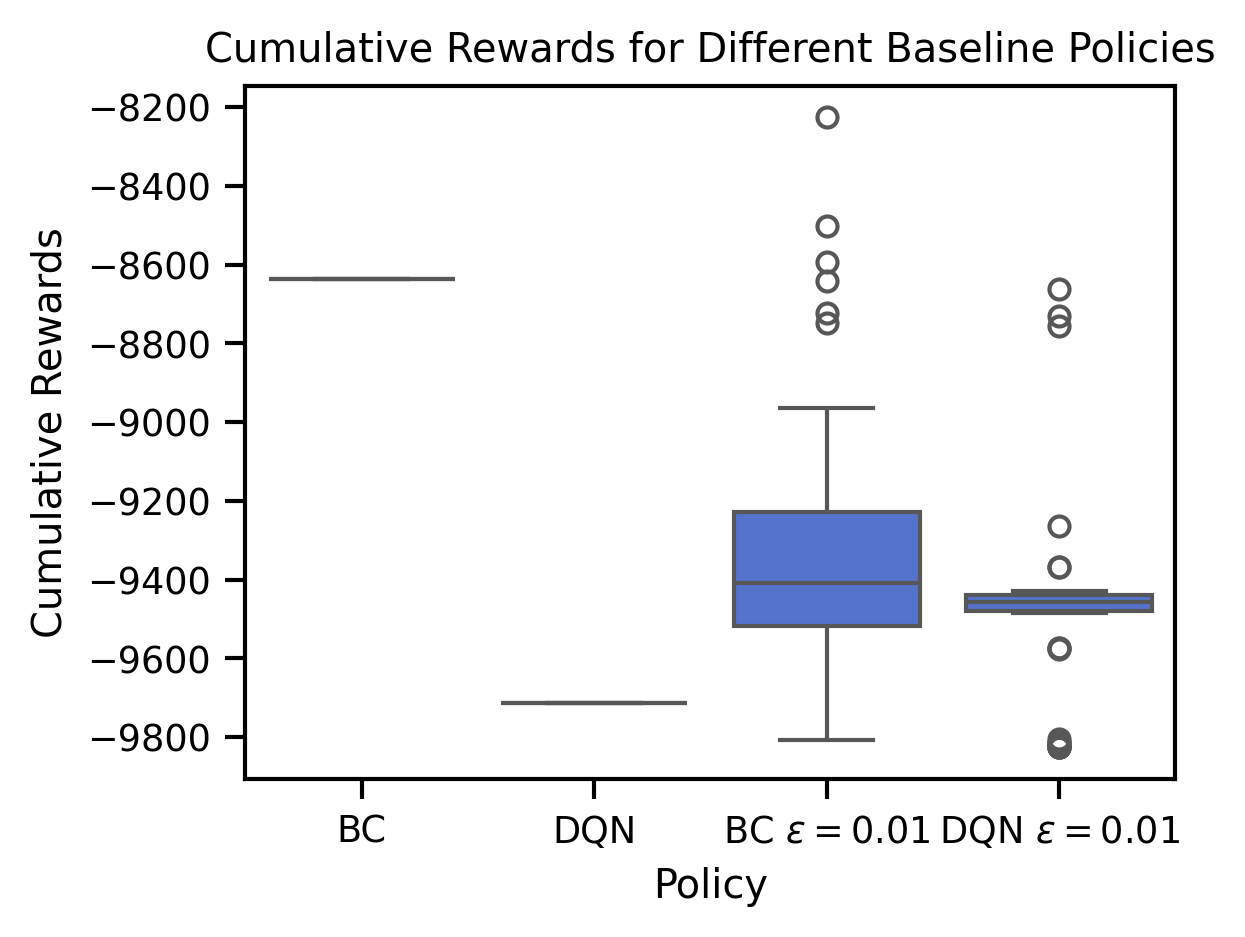
\includegraphics[width=0.8\columnwidth]{figures/cum_rewards_baseline.png}
      \vspace{0.5cm} % adjust vertical space as needed
      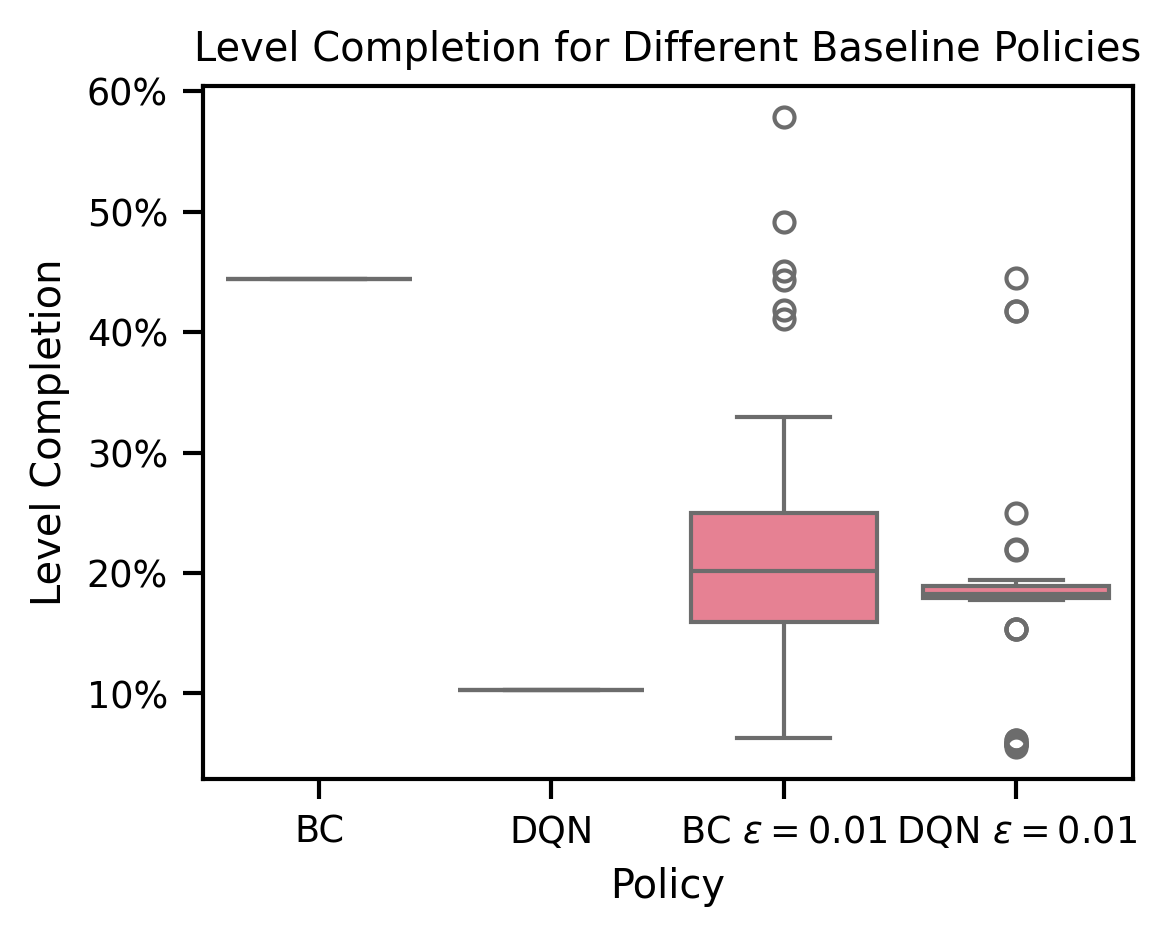
\includegraphics[width=0.8\columnwidth]{figures/completions_baseline.png}
      \caption{Baseline policies in-game performance statistics for 50 episodes each.}
      \label{fig:baseline_policies}
\end{figure}

DQN policy $\pi_{\text{DQN}}$ and BC policy $\pi_{\text{BC}}$ are learned 
through the aforementioned setups. It took about 8 hours to train 
$\pi_{\text{DQN}}$ and 1 hour for $\pi_{\text{BC}}$ on the GPU. After training, 
we rolled out 50 game plays for each policy to evaluate their performance based 
on cumulative rewards at terminated states and game completion percentage, 
defined as the total x-scrolling distance compared to the end of the level. 

Since the trained policies are deterministic, we introduce some stochasticity 
by adding a small $\epsilon=0.01$ where the policy will act randomly. This evaluates 
the robustness under perturbations, especially in complex game settings where 
encountering enemies and obtaining power-ups can significantly change the best 
actions to take. For all gameplays, the initial action is set to move right 
regardless of the policies to avoid Mario being stalled.

Both policies failed to complete the game level successfully.
$\pi_{\text{BC}}$ demonstrates significantly better performance in terms of 
cumulative rewards and game completions under the deterministic setup, despite 
taking only 1/8 of the time to train compared to $\pi_{\text{DQN}}$ and using 
only 5 human-demonstrated trajectories, as shown in Figure 
\ref{fig:baseline_policies}. However, $\pi_{\text{BC}}$ suffers from greater 
performance degradation when random perturbations are introduced. It exhibits 
higher variance in performance in stochastic setups.
$\pi_{\text{DQN}}$, on the other hand, is rather difficult to train. In the 
complex game environment, though rewards are not sparse, encountering enemies 
and power-ups makes the Markov assumptions less valid, and the pipes in the 
game create challenges for the agent to explore states effectively. Thus, the 
explorations are rarely sufficient to learn good $Q$ value estimations even 
after 2500 episodes (see Appendix \ref{a2:dqn}). The trained $\pi_{\text{DQN}}$ 
does not compare with $\pi_{\text{BC}}$ in deterministic settings but shows 
superior stability in terms of variance when randomness is introduced, with 
increased performance when acting stochastically. This illustrates that the 
current exploration is sub-optimal, and when exploring guided by human 
demonstrations, it could surpass $\pi_{\text{BC}}$ in performance.

\section{Next Steps}
Above initial results show the expected performance of baselines. The remaining 
work of the project involves finishing the implementation of the HRL algorithms 
and evaluating the performance of each approach.

\subsection{Deep \textit{Q}-Learning from Demonstrations (DQfD)}

Following the DQfD (Deep \textit{Q}-Learning from Demonstrations) framework by 
\cite{hester_dqfd_2017}, we incorporate human demonstrations into the replay 
buffer $\mathcal{D}$ of DQN to control explorations. This builds on the already 
implemented DQN framework, where the loss functions and replay buffer 
trajectories are modified to include human demonstrations.

\subsection{PPO with Behavior Cloning Warm-start}

Inspired by \cite{Coletti2023EffectivenessOW}, this approach leverages 
$\pi_{\text{BC}}$ trained model weights as a warm-start, then further leverages 
PPO for policy fine-tuning. PPO's property of 
prohibiting significant updates to the policies ensures that explorations will 
be around human demonstrations, with the possibility to improve and surpass 
human performance.

\subsection{Evaluations}
We will evaluate the approaches using both quantitative and qualitative metrics. 
Quantitatively, performance will be measured via cumulative reward, level 
completion rate, and distance traversed per episode, plotted as learning curves 
against training episodes or timesteps. Multiple independent runs will ensure 
statistical significance. Sample efficiency will be analyzed by measuring 
interactions required to reach performance thresholds and wall-clock training 
time. Qualitatively, gameplay visualizations and trajectory overlays will 
provide insights into behavioral strategies.


\bibliography{ref}
\bibliographystyle{icml2018}

\clearpage
\appendix
\renewcommand{\thefigure}{A\arabic{figure}}
\renewcommand{\thetable}{A\arabic{table}}
\setcounter{figure}{0}
\setcounter{table}{0}
\onecolumn
\section{Appendix}
\subsection{Custom Environment}
\label{a1:custom_env}

The default 512 discrete action space captures all possible joystick button 
combinations. However, most of these combinations are not meaningful for 
controlling Mario. From the human demonstration trajectories, we narrowed down 
the action space to 10 common used button combinations.
Then the action vector is labeled as integers (0-9, following below orders)
as discrete action space for the environment.

\begin{verbatim}
# List of meaningful button combinations used in gameplay
meaningful_actions = [
      [0, 0, 0, 0, 0, 0, 0, 0, 0],  # No action
      [0, 0, 0, 0, 0, 0, 0, 0, 1],  # A (Jump)
      [0, 0, 0, 0, 0, 0, 0, 1, 0],  # Right
      [0, 0, 0, 0, 0, 0, 0, 1, 1],  # Right + A (Jump)
      [0, 0, 0, 0, 0, 0, 1, 0, 0],  # Left
      [0, 0, 0, 0, 0, 0, 1, 0, 1],  # Left + A (Jump)
      [1, 0, 0, 0, 0, 0, 0, 0, 0],  # B (Run)
      [1, 0, 0, 0, 0, 0, 0, 0, 1],  # A + B (Jump + Run)
      [1, 0, 0, 0, 0, 0, 0, 1, 0],  # Right + B (Run)
      [1, 0, 0, 0, 0, 0, 0, 1, 1]   # Right + A + B (Jump + Run)
]
\end{verbatim}

\subsection{DQN Training}
\label{a2:dqn}

$\pi_{\text{DQN}}$ is rather difficult to train. In the 
complex Super Mario Bros game environment, though rewards are not sparse, encountering enemies 
and power-ups makes the Markov assumptions less valid, and the pipes in the 
game create challenges for the agent to explore states effectively.

As seen in Figure \ref{figa:dqn}, the loss has increased as random explorations 
reduced. The rewards grow very slowly and drastically drop at the end. We 
observed the policy was stuck in a reward-hacking phase where Mario moves only 
to the left until time-out termination. This reduces the risks of getting stuck 
at further pipes with lower rewards and encountering enemies. Such behaviors 
might be addressed by tuning reward functions and exploring if HRL can help 
with this situation.

\begin{figure}[htbp]
\centering
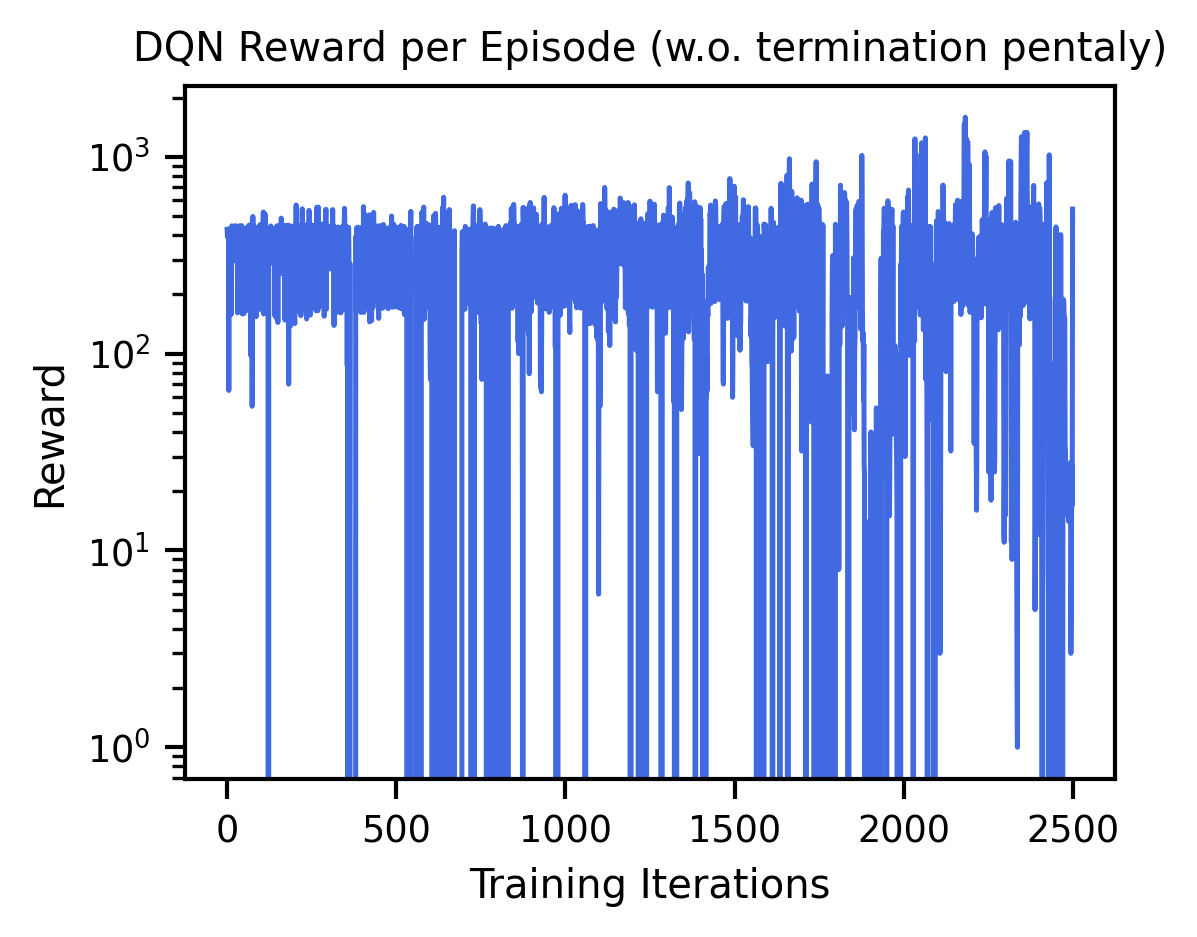
\includegraphics[width=0.45\columnwidth]{figures/dqn_rewards.png}
\hspace{0.5cm} % adjust horizontal space as needed
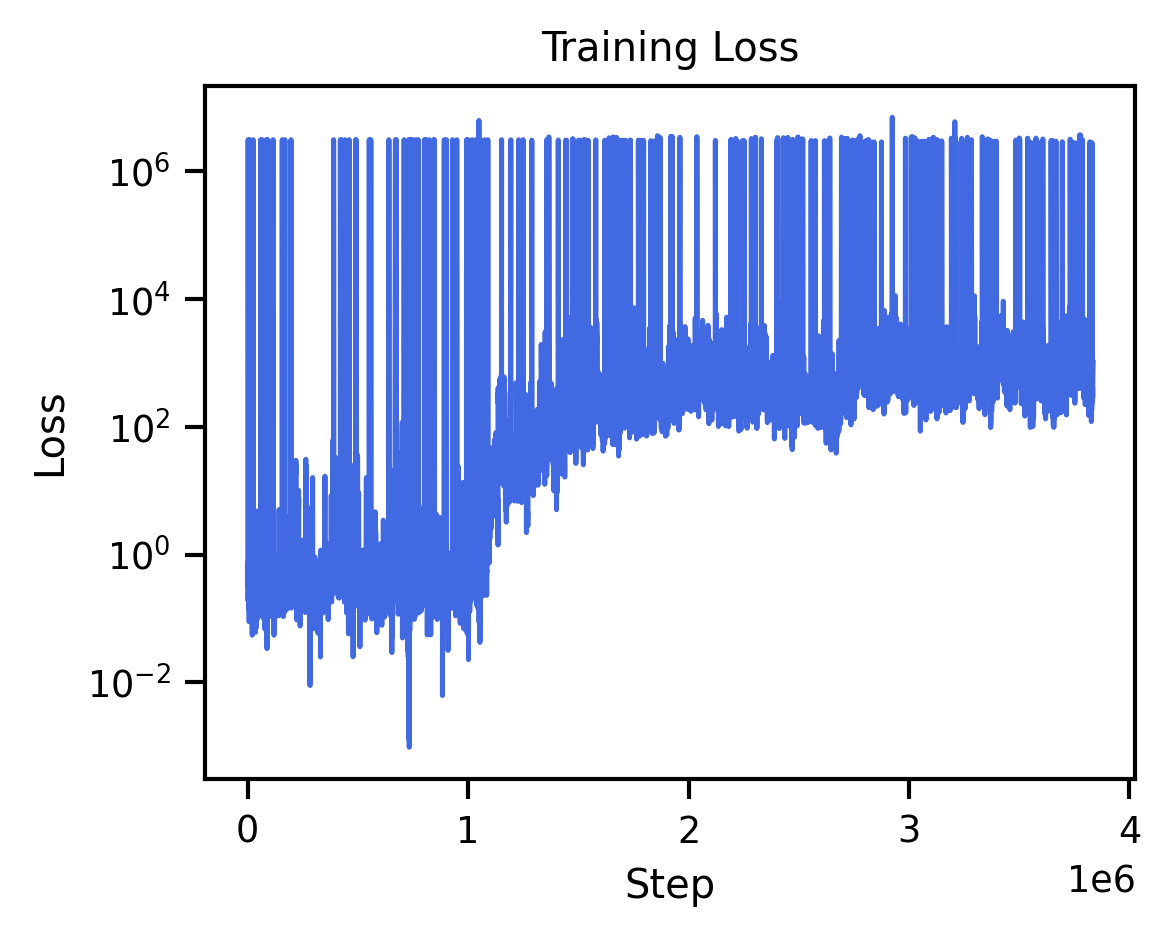
\includegraphics[width=0.45\columnwidth]{figures/dqn_loss.png}
\caption{DQN training loss and rewards}
\label{figa:dqn}
\end{figure}



\end{document}